\documentclass[a4paper,11pt]{article}
\pdfoutput=1 % if your are submitting a pdflatex (i.e. if you have
             % images in pdf, png or jpg format)

\usepackage{jheppub} % for details on the use of the package, please
                     % see the JHEP-author-manual

\usepackage[T1]{fontenc} % if needed
\usepackage{amsmath}
\usepackage{leftidx}
\usepackage{multirow}
\title{\boldmath  Flavour Symmetry Embedded - GLoBES}



% more complex case: 4 authors, 3 institutions, 2 footnotes
\author[a]{Jian Tang,}
\author[a]{Tse-Chun Wang}


% The "\note" macro will give a warning: "Ignoring empty anchor..."
% you can safely ignore it.

\affiliation[a]{School of Physics, Sun Yat-Sen University, Guangzhou 510275, China}
%\affiliation[c]{A School for Advanced Studies,\\some-location, Country}

% e-mail addresses: one for each author, in the same order as the authors
\emailAdd{tangjian5@mail.sysu.edu.cn}
\emailAdd{wangzejun@mail.sysu.edu.cn}




\abstract{Abstract...}



\begin{document} 
\maketitle
\flushbottom

\section{Introduction}\label{sec:intro}
{\color{red}intro flavour symmetry, and summarise some phenon works}


The discovery of neutrino oscillations points out the fact that neutrinos have mass, and provides evidence beyond the Standard Model (BSM). This phenomenon is successfully described by a theoretical framework with the help of three neutrino mixing angles ($\theta_{12}$, $\theta_{13}$, $\theta_{23}$), two mass-square splittings ($\Delta m_{21}^2$, $\Delta m_{31}^2$), and one Dirac CP phase ($\delta$) \cite{Pontecorvo:1967fh,Maki:1962mu,Pontecorvo:1957qd,Esteban:2018azc}. Thanks to the great efforts in the past two decades, we almost have a complete understanding of such a neutrino oscillation framework. More data in the neutrino oscillation experiments is needed to determine the sign of $\Delta m_{31}^2$, to measure the value of $\sin\theta_{23}$, to discover the potential CP violation in the leptonic sector and even to constrain the size of $\delta$ \cite{Esteban:2018azc}. For these purposes, the on-going long baseline experiments (LBLs), such as the NuMI Off-axis $\nu_e$ Appearance experiment (NO$\nu$A)~\cite{Ayres:2007tu} and the Tokai-to-Kamioka experiment (T2K)~\cite{Abe:2011ks}, can answer these questions with the statistical significance $\gtrsim 3\sigma$ in most of the parameter space. Based on the analysis with their data, the normal mass ordering ($\Delta m_{31}^2>0$), the higher $\theta_{23}$ octant ($\theta_{23}>45^\circ$), and $\delta\sim270^\circ$ are preferred so far~\cite{Esteban:2018azc}. The future LBLs, Deep Underground Neutrino Experiment (DUNE)~\cite{Acciarri:2015uup}, Tokai to Hyper-Kamiokande (T2HK)~\cite{Abe:2014oxa}, and the medium baseline reactor experiment, the Jiangmen Underground Neutrino Observatory (JUNO)~\cite{Djurcic:2015vqa,An:2015jdp} will further complete our knowledge of neutrino oscillations.

Flavour symmetry models are used to explain the origin of the neutrino mixing, and to predict the value of oscillation parameters (some of useful review articles are~\cite{Altarelli:2010gt,Ishimori:2010au,King:2013eh,King:2014nza,King:2015aea,King:2015ata,King:2017guk}). These models are motivated by some interesting features, \textit{such as} $\theta_{12}\sim 33^\circ$, and $\theta_{23}\sim 45^\circ$. Before the discovery of non-zero $\theta_{13}$ measurement by Daya Bay experiment~\cite{An:2013zwz}, the `tri-bi-maximal' neutrino mixing (TBM) ansatz, which was proposed in 2002 by Horrison, Perkins, and Scott~\cite{Harrison:2002er}, fitted with the experimental data in a good agreement:
\begin{equation*}
U_{\text{TBM}}=\left(
\begin{array}{ccc}
2/\sqrt{6} & 1/\sqrt{3} & 0\\
-1/\sqrt{6} & 1/\sqrt{3} & 1/\sqrt{2}\\
1/\sqrt{6}  & -1/\sqrt{3} & 1/\sqrt{2}
\end{array}\right).
\end{equation*} 
With the fact that $\theta_{13}\approx 8^\circ$, several ways to obtain such non-zero value of $\theta_{13}$ are proposed. One of popular proposals is to correct the tri-bi-maximal neutrino mixing such that 
\begin{equation*}
\sin\theta_{12}=(1+s)/\sqrt{3},~\sin\theta_{13}=r/\sqrt{2},~\text{and}~\sin\theta_{23}=(1+a)/\sqrt{2}.
\end{equation*}
Th neutrino mixing ansatz can be realised by high-energy symmetries $G_f$.
The symmetry of discrete groups $G_f$, preserved at the high energy but slightly broken at the lower energy, predicts the neutrino mixing, mass-square splittings, and the CP violation phase (Dirac and Majorana phases), with reduced degrees of freedom. 
The symmetries need to be broken at the low energy. Otherwise, the flavour of leptons cannot be distinguished. There are several approaches for the symmetry breaking, including the direct, indirect, and semi approaches. Direct approach preserves the residual symmetries of $G_f$ in the charged-lepton or neutrino sector. On the other hand, there is no residual symmetry preserved in neither charged-lepton nor neutrino sector in the indirect approach. In the semi approach, the charged-lepton and neutrino sectors preserve different residual symmetries, respectively. This symmetry is broken by extending the Higgs sector or introducing the flavons.
%As a result, these models do not only simplify the theoretical framework for neutrino oscillations, but also provide a theoretical reason for this phenomenon. Many of these models can well describe the current neutrino-oscillation data. 
%
To achieve the $\delta$ prediction, many models are based on a discrete family symmetry $G_f$ together with a non-commuting CP symmetry $H_\mathrm{CP}$. Broken in different approaches, the symmetry $G_f\otimes H_\mathrm{CP}$ can predict different patterns for the neutrino mixing. For example, in the semi-direct approach, $S_4$ is preserved in the leading order, and leads the bimaximal (MB) or tri-bimaximal (TB) neutrino mixing, while the higher order terms bring the correction to the neutrino mixing.

Currently, some works discuss on how the future experiments can be used for testing these flavour symmetry models in the phenomenological point of view, \textit{e.g.}~\cite{Ballett:2016yod,Chatterjee:2017xkb,Ding:2019zhn,Tang:2019edw}. A large number of these works are based on the \texttt{c}-library -- \textbf{G}eneral \textbf{Lo}ng \textbf{B}aseline \textbf{E}xperiment \textbf{S}imulator (\textbf{GLoBES}) \cite{Huber:2004ka,Huber:2007ji}, which is a convenient simulation tool to simulate neutrino oscillation experiments via the Abstract Experiment Definition Language (AEDL). Some AEDL files for experiments are also available on \textbf{GLoBES} website. In addition, the working group of DUNE experiment also releases their AEDL files~\cite{Alion:2016uaj}.  \textbf{GLoBES} can be taken as one of popular and useful tools in the community of neutrino oscillation physics. However, it has not yet to be extended for the purpose of analysing flavour symmetry models. 

In this work, we will present our simulation tool \textbf{F}l\textbf{a}vour \textbf{S}ymmetry \textbf{E}mbedded - \textbf{GLoBES} (\textbf{FaSE-GloBES}) that is a simulation code based on GLoBES library and specific for studying the flavour symmetry. 

%One of the most predictive flavour-symmetry models is the littlest seesaw model (LSS), which includes two massive right-handed neutrinos: one corresponds to the atmospheric-mass term, while the other is included for the solar-mass term~\cite{King:2013iva,King:2015dvf,King:2016yvg}.  The littlest seesaw model in the tri-direct approach (TDLS) has been proposed and succeeds in describing the current global-fit results~\cite{Ding:2018fyz,Ding:2018tuj}. The tri-direct approach is that after the breaking of the family symmetry $G_f\otimes H_\mathrm{CP}$, three residual symmetries are preserved in different sectors: one in the charged-lepton sector, two in the sectors of right-handed neutrinos for atmospheric and solar mass terms, respectively. In this model, four parameters $x$, $\eta$, $r$, $m_a$ are used to describe neutrino oscillations. This model has been studied with simulated data at NO$\nu$A, T2K, DUNE, T2HK and JUNO~\cite{Ding:2019zhn}. In this work, we study how the next-generation neutrino project using muon-decay beams such as MOMENT can further extend our knowledge on the TDLS model. We have two reasons to motivate this study. Firstly, TDLS describes the current data successfully and tends to be a nice way to offer neutrino mass terms from theoretical point of view. Secondly, it must be straightforward to test the underlying model predictions and compare the performance of MOMENT to the other experiments, \textit{such as} NO$\nu$A, T2K, DUNE, and T2HK.


\section{Overview FASE-GloBES}

\begin{figure}[!h]%
\centering
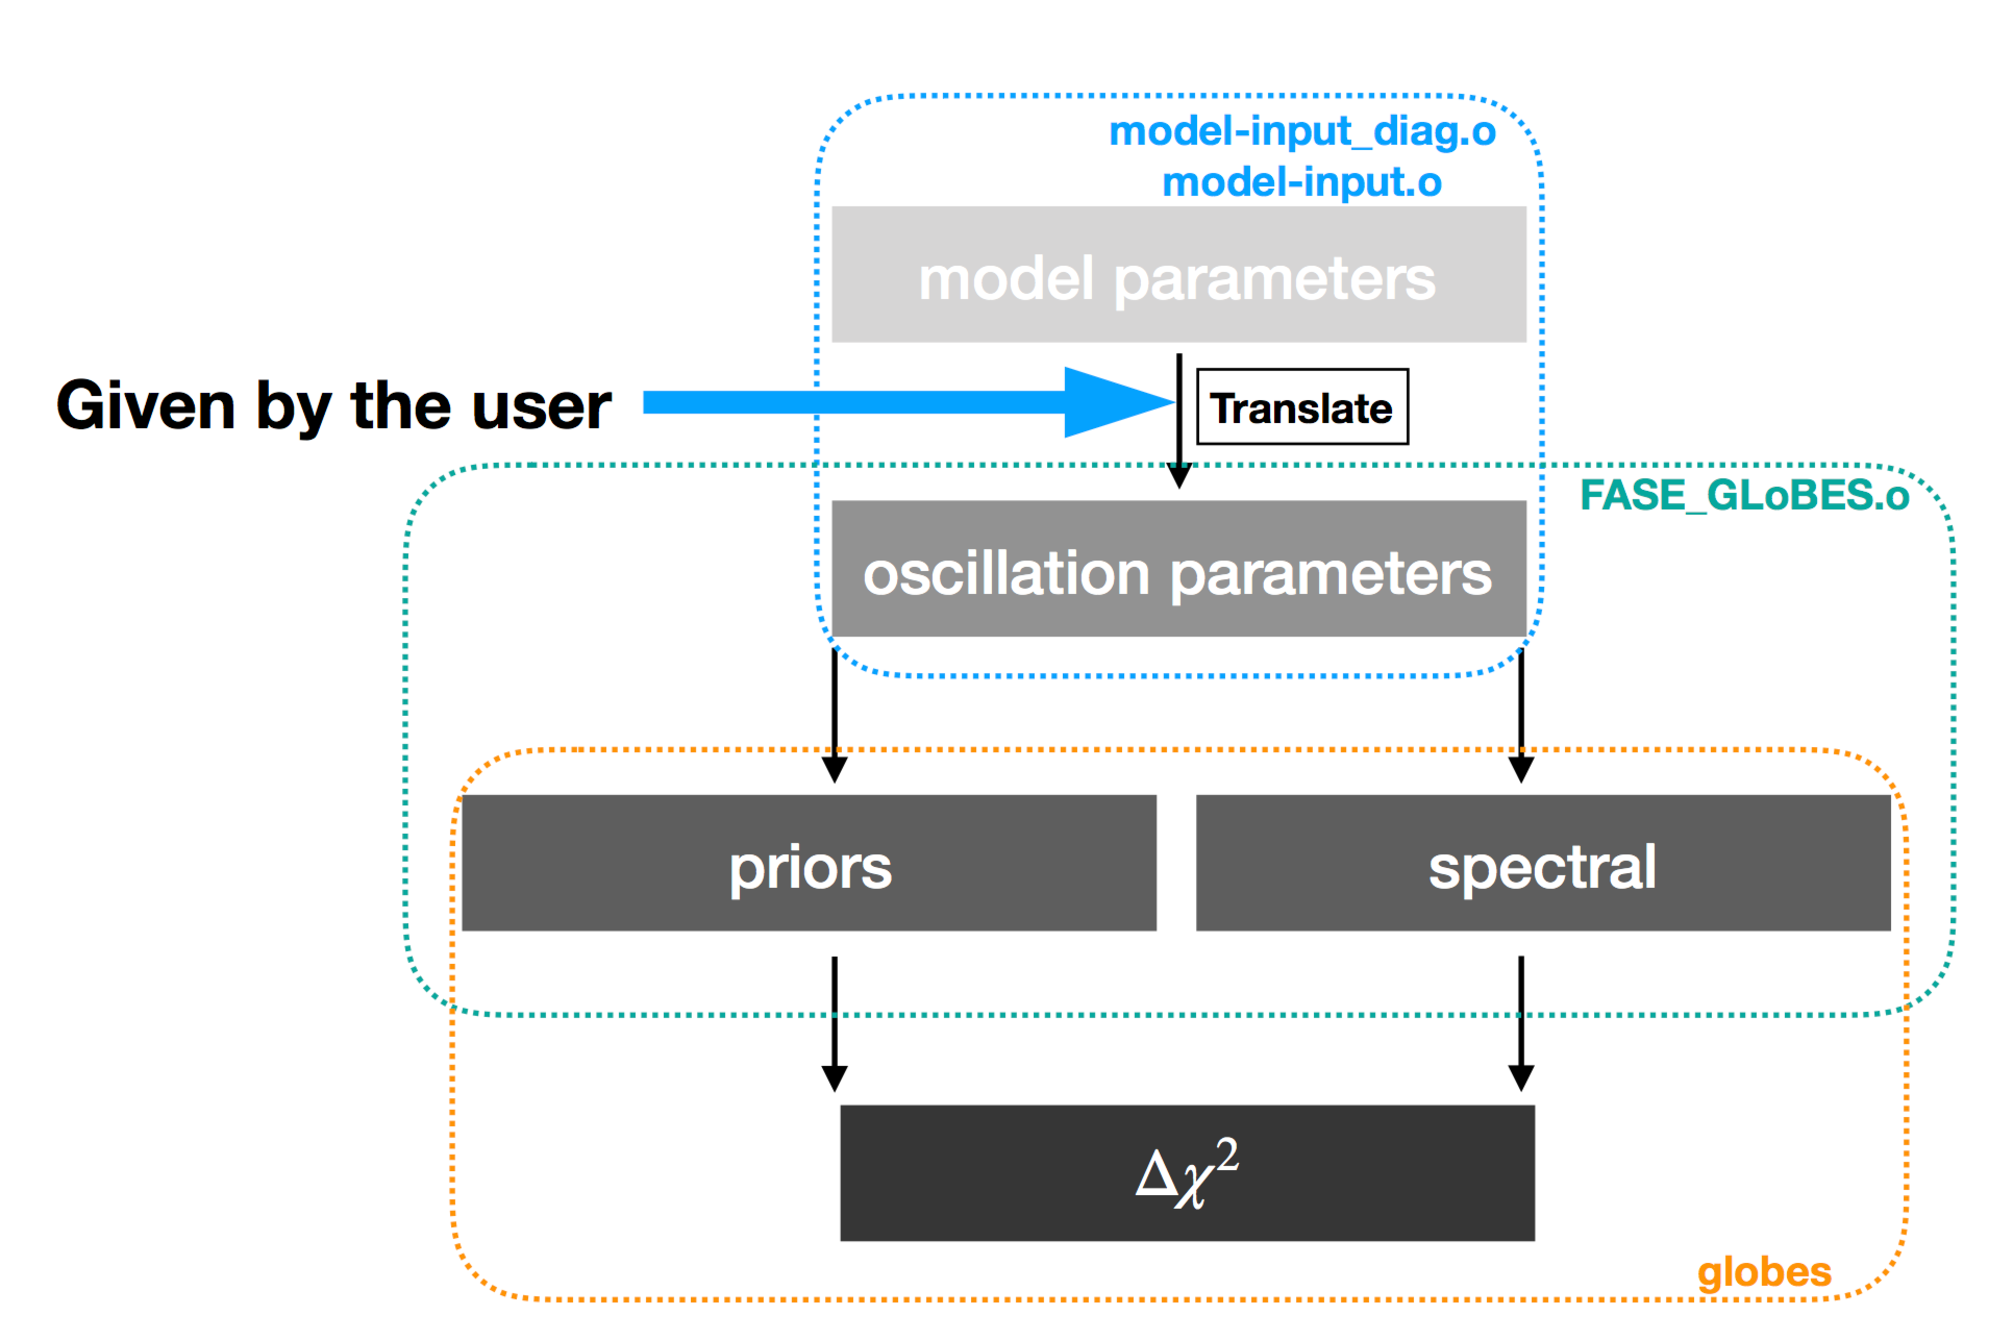
\includegraphics[width=5in]{Figs/FASE-chart-1_v1.pdf}
\caption{A scheme to correlate the model parameters with standard neutrino oscillation parameters. The error propagation is implemented in the simulation code up to the spectra analysis.}%
\label{fig:FASE}
\end{figure}

The FASE-GLoBES is based on GLoBES as shown in Fig.~\ref{fig:FASE}, in which three parts are shown: 1. \textbf{the parameter translation} (the blue box), 2. \textbf{giving oscillation-parameter values} (the green box), and 3. \textbf{the $\chi^2$-value calculation} (the orange box). 
The idea behind this flow chart Fig.~\ref{fig:FASE} is that given a set of value for model parameter, the corresponding values for oscillation parameters are obtained by a translation, which is assigned by the user in \textbf{model-input\_diag.c} or \textbf{model-input.c}. And then, through \textbf{FASE\_GLoBES.c}, these oscillation-parameter values are passed in to \textbf{GLoBES} library to simulate the event spectrum for evaluating the $\chi^2$ value. Using prior needs 

In the following, we give more details about using FASE-GLoBES. In Sec.~\ref{sec:download}, we will give the instruction to download and install GLoBES and FASE-GLoBES. Then, in Sec.~\ref{sec:compile}, we will introduce how to compile and run the code. More complicated is setting the model, and the way to do this will be described in Sec.~\ref{sec:model_set}. Finally, we will discuss how to set up the prior in Sec.~\ref{sec:prior}.



\subsection{Download and Installation}\label{sec:download}
\textbf{download and install GLoBES and FASE-GLoBES}\\
{\color{red}[will fill in after the code ready on Github]}

\subsection{Compile and Run}\label{sec:compile}
{\color{red}[will fill in after the code ready on Github]}

To initial \textbf{FASE-GLoBES}, we need to include the following code\\
\texttt{    MODEL\_init($N_{para}$); }\\
where $N_{para}$ is the number of model parameters.

\subsection{Model setting}\label{sec:model_set}

FASE includes three \texttt{c++} files: \textbf{model-input\_diag.c}, \textbf{model-input.c}, and \textbf{FASE\_GLoBES.c}. As shown in the previous paragraph, these files are for different service. In \textbf{model-input\_diag.c} and \textbf{model-input.c}, the user can assign the relation between the oscillation and model parameter sets. The difference between these two code is that in \textbf{model-input.c}, the user give the relation between these two parameter sets directly (\textit{e.g.}~Table~\ref{tab:TD_parameters} for tri-direct littlest seesaw), while in \textbf{model-input.c}, the mass matrix (\textit{e.g.}~Eq.~\ref{eq:mnu} for tir-direct littlest seesaw), which is provided by the user, can be diagonalised to obtain the corresponding oscillation-parameter values. 

We now take the littlest seesaw model in the tri-direct approach as an example. In this model, the atmospheric and solar flavon vacuum alignments are $\langle\phi_{\text{atm}}\rangle\propto\left(1, \omega^2, \omega\right)^T$ and $\langle\phi_{\text{sol}}\rangle\propto\left(1, x, x\right)^T$,
where  stands for a cube root of unity and the parameter $x$ is real because of the imposed CP symmetry. Under this model, the light left-handed Majorana neutrino mass matrix is given by
\begin{equation}
\label{eq:mnu}  m_{\nu}=m_{a}\begin{pmatrix}
 1 &~ \omega  &~ \omega ^2 \\
 \omega  &~ \omega ^2 &~ 1 \\
 \omega ^2 &~ 1 &~ \omega  \\
\end{pmatrix}+e^{i\eta}m_{s}
\begin{pmatrix}
 1 &~  x &~  x \\
 x &~ x^2 &~ x^2 \\
 x &~ x^2 &~ x^2 \\
\end{pmatrix}\,,
\end{equation}
where $x$, $\eta$, $m_a$, and the ratio $r\equiv m_s/m_a$ are four parameters and will be constrained by experimental data. We note that from Eq.~(\ref{eq:mnu}), $m_1=0$ and the normal mass ordering are imposed, and will need to be imposed in \textbf{FASE-GLoBES}. We will introduce the way to do it in Sec.~\ref{sec:prior}.

\begin{table}[h!]
\caption{\label{tab:TD_parameters}A summary of the relation between oscillation parameters and TDLS model parameters~\cite{Ding:2018fyz}. Two requirements are imposed by TDLS: the smallest mass state $m_1=0$ and the normal mass ordering. The sign of $\sin\delta$ depends on the sign of $x\cos\psi$: ``$+$'' (``$-$'') is for $x\cos\psi>0$ ($<0$).}
\begin{tabular}{l|l}
\hline\hline
model parameters                                 & $x$, $\eta$, $r$, $m_a$                                                                                                                                                                         \\\hline
\multirow{6}{*}{combinations of model parameters} & $y=\frac{5x^2+2x+2}{2\left(x^2+x+1\right)}(m_{a}+e^{i \eta } m_{s})$,                                                                                                                            \\
                                                 & $z=-\frac{\sqrt{5x^2+2x+2}}{2\left(x^2+x+1\right)}\left[ (x+2)m_{a}-x(2x+1)e^{i \eta }m_{s}\right]$,                                                                                             \\
                                                 & $w=\frac{1}{2(x^2+x+1)}\left[(x+2)^2m_{a}+x^2\left(2x+1\right)^2e^{i \eta } m_{s}\right]$,                                                                                                       \\
                                                 & $\sin\psi=\frac{\Im\left(y^{*}z+wz^{*}\right)}{|y^{*}z+wz^{*}|},\quad \cos\psi=\frac{\Re\left(y^{*}z+wz^{*}\right)}{|y^{*}z+wz^{*}|}$.                                                           \\
                                                 & \begin{tabular}[c]{@{}l@{}}$\sin2\theta=\frac{2|y^{*}z+wz^{*}|} {\sqrt{(|w|^2-|y|^2)^2+4|y^{*}z+wz^{*}|^2}},$\end{tabular}                                                                     \\
                                                 & $\cos2\theta=\frac{|w|^2-|y|^2}{\sqrt{(|w|^2-|y|^2)^2+4|y^{*}z+wz^{*}|^2}}$.                                                                                                                     \\\hline
\multirow{7}{*}{oscillation parameters}          & $\Delta m_{21}^2=m^2_2=\frac{1}{2}\left[\left|y\right|^2+\left|w\right|^2+2\left|z\right|^2-\frac{\left|w\right|^2-\left|y\right|^2}{\cos\theta}\right]$,                                        \\
                                                 & $\Delta m_{31}^2=m^2_3=\frac{1}{2}\left[\left|y\right|^2+\left|w\right|^2+2\left|z\right|^2+\frac{\left|w\right|^2-\left|y\right|^2}{\cos\theta}\right]$,                                        \\
                                                 & $\sin^2\theta_{12}=1-\frac{3x^2 }{3x^2+2\left(x^2+x+1\right) \cos^2\theta }$,                                                                                                                  \\
                                                                                                  & $\sin^2\theta_{13}=\frac{2\left(x^2+x+1\right)\sin^2\theta}{5x^2+2x+2}$,                                                                                                                       \\
                                                 & $\sin^2\theta_{23}=\frac{1}{2}+\frac{x\sqrt{3\left(5x^2+2x+2\right)}\sin2\theta\sin\psi }{2\left[3x^2+2\left(x^2+x+1\right) \cos^ 2 \theta\right]}$,                                          \\
                                                 & $\cos\delta=\frac{ \cot 2 \theta_{23} \left[3x^2-\left(4x^2+ x+1\right)\cos^2\theta_{13}\right]}{\sqrt{3} \left|x\right| \sin \theta_{13} \sqrt{\left(5x^2+2x+2\right)\cos^2\theta_{13}-3x^2}}$, \\
                                                 & $\sin\delta= \pm\csc 2 \theta_{23} \sqrt{1+\frac{\left(x^2+x+1\right)^2 \cot ^2\theta_{13} \cos ^22 \theta_{23}}{3x^2 \left[3x^2 \tan ^2\theta_{13}-2 \left(x^2+x+1\right)\right]}}$.   \\\hline \hline       
\end{tabular}
\end{table}


For different methods to include the model, we use different \texttt{c++} file. Adopting the mass matrix Eq.~\ref{eq:mnu}, we assign this model in \textbf{model-input\_diag.c}. In function \texttt{MtoS}, we give
the mass matrix Eq.~\ref{eq:mnu} in the $3\times3$ complex matrix \texttt{Mass\_Matrix[]}.\vspace{0.5cm}

\texttt{int MtoS(double OSC\_PARAMS[6],~double M\_para[])}\\
\texttt{\{}
\\        
   \texttt{double x=M\_para[0];}\\
    \texttt{double eta=M\_para[1];}\\
    \texttt{double r=M\_para[2];}\\
    \texttt{double ma=M\_para[3];}\\
    \texttt{double ms=ma*r;}\\
    
    \texttt{double complex Mass\_Matrix[] = \{ma+ms*(cos(eta) + I*sin(eta)), ma*(cos(6.6666e-1*M\_PI) + I*sin(6.6666e-1*M\_PI))+x*ms*(cos(eta) + I*sin(eta)), ma*(cos(6.6666e-1*M\_PI) + I*sin(6.6666e-1*M\_PI))*(cos(6.6666e-1*M\_PI) + I*sin(6.6666e-1*M\_PI))+x*ms*(cos(eta) + I*sin(eta)), ma*(cos(6.6666e-1*M\_PI) + I*sin(6.6666e-1*M\_PI))+x*ms*(cos(eta) + I*sin(eta)), ma*(cos(6.6666e-1*M\_PI) + I*sin(6.6666e-1*M\_PI))*(cos(6.6666e-1*M\_PI) + I*sin(6.6666e-1*M\_PI))+x*x*ms*(cos(eta) + I*sin(eta)), ma+x*x*ms*(cos(eta) + I*sin(eta)), ma*(cos(6.6666e-1*M\_PI) + I*sin(6.6666e-1*M\_PI))*(cos(6.6666e-1*M\_PI) + I*sin(6.6666e-1*M\_PI))+x*ms*(cos(eta) + I*sin(eta)), ma+x*x*ms*(cos(eta) + I*sin(eta)), ma*(cos(6.6666e-1*M\_PI) + I*sin(6.6666e-1*M\_PI))+x*x*ms*(cos(eta) + I*sin(eta))\};}\\
    
    \texttt{STAN\_OSC(Mass\_Matrix,OSC\_PARAMS);}\\
    
    \texttt{return 0;}\\
\texttt{\} }

Passing the complex matrix \texttt{Mass\_Matrix[]} into the function \texttt{STAN\_OSC}, we will get the corresponding oscillation parameters in an array \texttt{OSC\_PARAMS}, components of which are the value for $\theta_{12}$, $\theta_{13}$, $\theta_{23}$, $\delta$, $\Delta m_{21}^2$, and $\Delta m_{31}^2$. The expression of \texttt{Mass\_Matrix[]} is given by the user. For the first four components, values are given in the unit of \textbf{rad}, while the other two are in eV$^2$. 


We can also assign the relation between oscillation and model parameters Table~\ref{tab:TD_parameters} in \textbf{model-input.c}. The relations are given in \texttt{MtoS} as well.\vspace{0.5cm}

\texttt{double MtoS(double osc\_para[6], double M\_para[])}\\
\texttt{\{}\\
    \texttt{/*example: tri-direct*/}\\
\\    
    \texttt{double x\_in   = M\_para[0];}\\
    \texttt{double eta\_in = M\_para[1];}\\
    \texttt{double r\_in   = M\_para[2];}\\
    \texttt{double ma\_in  = M\_para[3];}\\
\\  
    \texttt{osc\_para[0]=TDth12(x\_in,eta\_in,r\_in, ma\_in);}\\
    \texttt{osc\_para[1]=TDth13(x\_in,eta\_in,r\_in, ma\_in);}\\
    \texttt{osc\_para[2]=TDth23(x\_in,eta\_in,r\_in, ma\_in);}\\
    \texttt{osc\_para[3]=TDdCP(x\_in,eta\_in,r\_in, ma\_in);}\\
    \texttt{osc\_para[4]=TDdm21(x\_in,eta\_in,r\_in, ma\_in);}\\
    \texttt{osc\_para[5]=TDdm31(x\_in,eta\_in,r\_in, ma\_in);}\\
\\    
    \texttt{return 0;}\\
\texttt{\}}\\

The functions \texttt{TDth12}, \texttt{TDth13}, \texttt{TDth23}, \texttt{TDdCP}, \texttt{TDdm21}, and \texttt{TDdm31} are included for obtaining the value of $\theta_{12}$, $\theta_{13}$, $\theta_{23}$, $\delta$, $\Delta m_{21}^2$, and $\Delta m_{31}^2$ according to Table~\ref{tab:TD_parameters}, respectively. 


\subsection{Prior setting}\label{sec:prior}
The \texttt{c++} file \textbf{FASE\_GLoBES.c} then will call these oscillation-parameter values and pass these to simulate the event spectrum. The $\chi^2$ value from priors is also given in \textbf{FASE\_GLoBES.c}. And these functions are given by the user.

\subsection{Summary of API}

\section{Examples}
\subsection{Constraint of model parameters}
%\subsection{Projection on the PMNS parameters}
\begin{figure}[!h]%
\centering
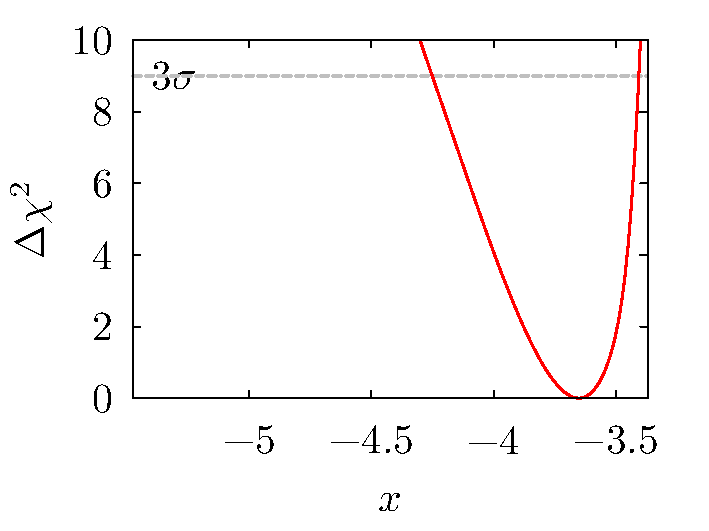
\includegraphics[width=2in]{figs/x.pdf}
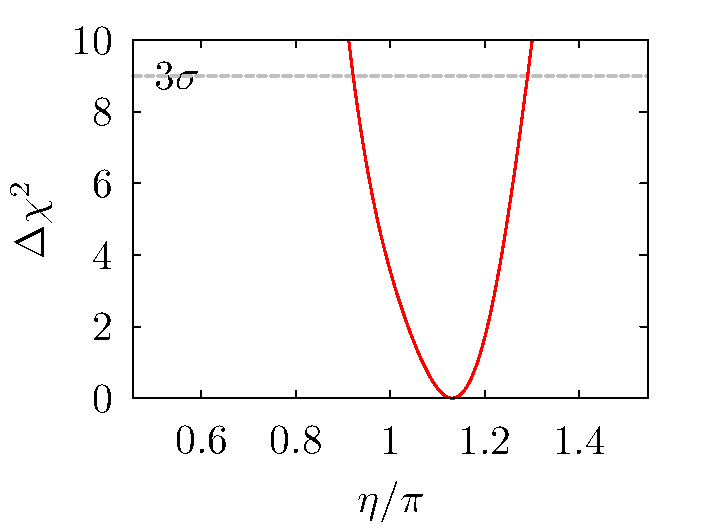
\includegraphics[width=2in]{figs/eta.pdf}\\
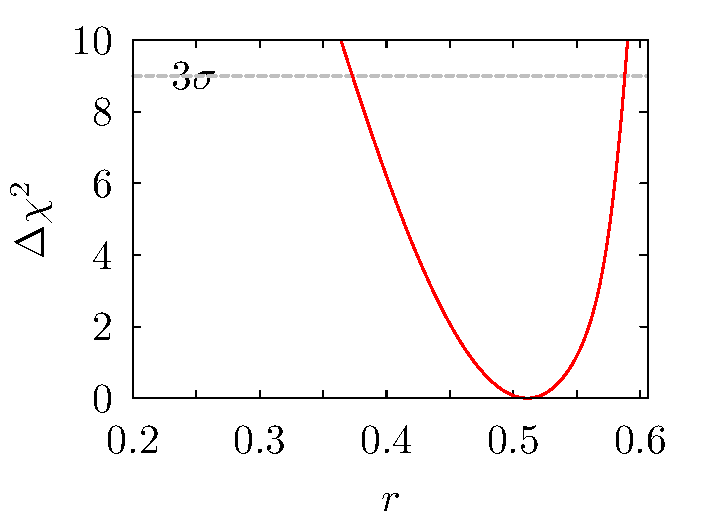
\includegraphics[width=2in]{figs/r.pdf}
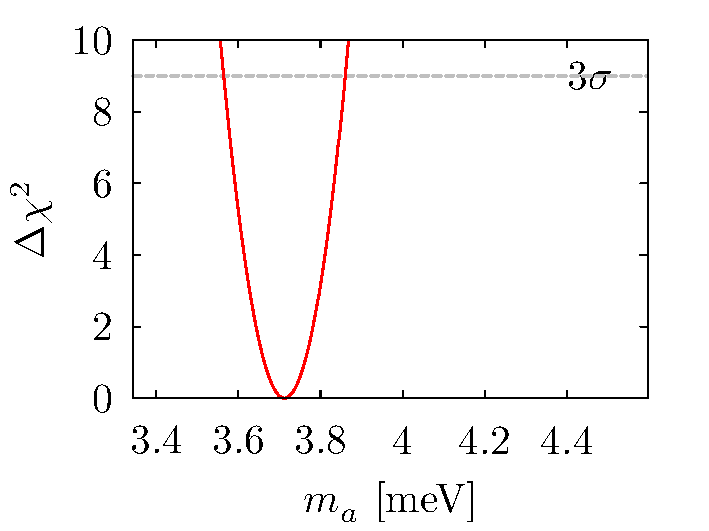
\includegraphics[width=2in]{figs/ma.pdf}
\caption{The $\Delta\chi^2$ value against each model parameters for MOMENT. True values for the model parameters are used $(x,~\eta,~r,~M_a)=(-3.65,~1.13\pi,~0.511,~3.71~\text{meV})$. The range shown here is according to the $3\sigma$ uncertainty with NuFit4.0 results:  $-5.475<x<-3.37$ (red band),~$0.455<\eta/\pi<1.545$ (dark grey band), ~$0.204<r<0.606$ (blue band),~$3.343<m_a/\text{meV}<4.597$ (yellow band).}%
\label{fig:model_1D}
\end{figure}

\begin{figure}[!h]
 \flushleft
\hspace{15mm}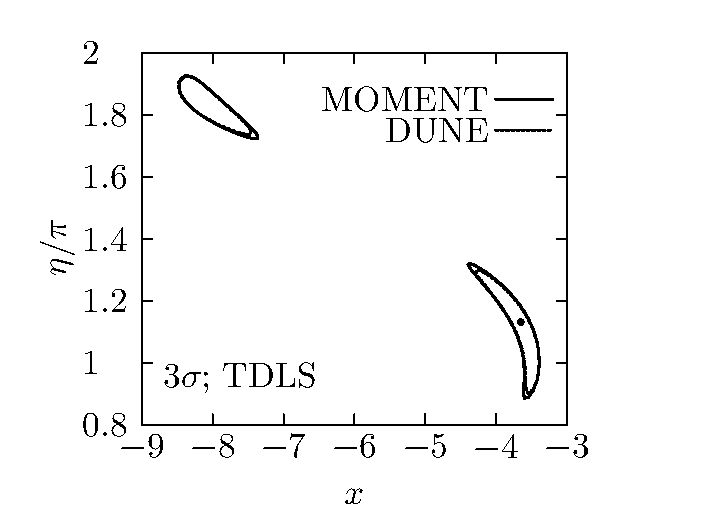
\includegraphics[width=0.32\textwidth]{figs/x_eta.pdf}$~~~~~~$\\
\hspace{15mm} 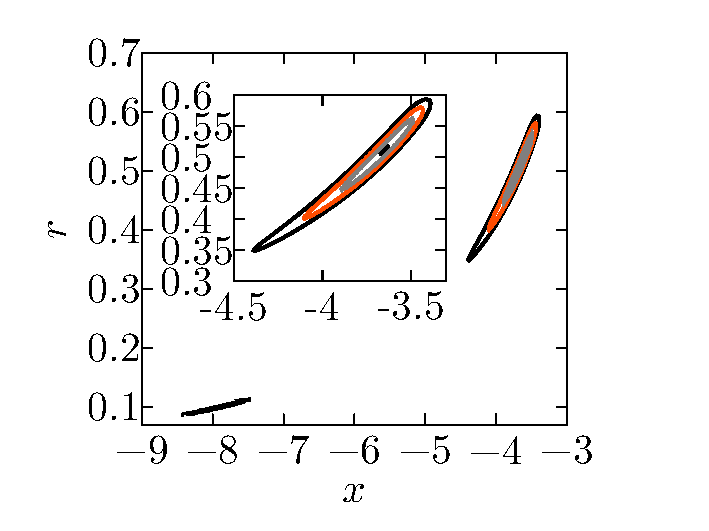
\includegraphics[width=0.32\textwidth]{figs/x_r.pdf}\hspace{-11mm}
 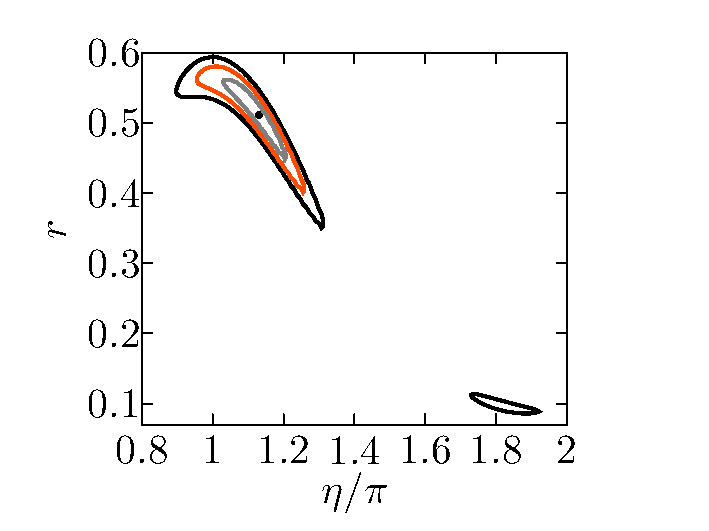
\includegraphics[width=0.32\textwidth]{figs/eta_r.pdf}$~~~~~~$\\
\hspace{15mm} 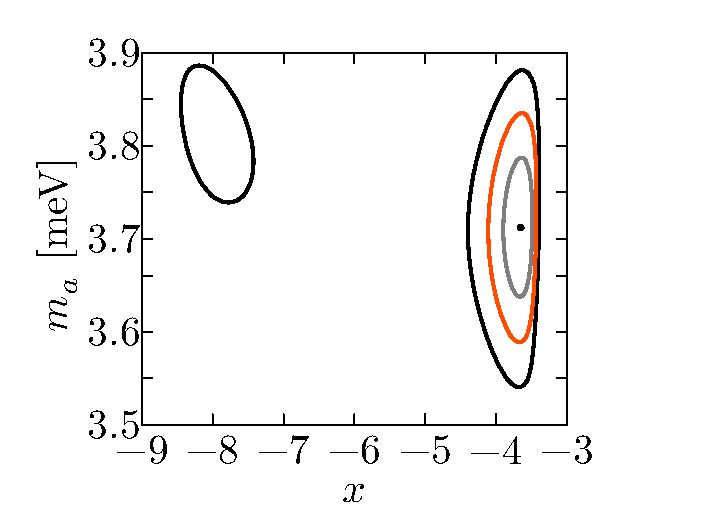
\includegraphics[width=0.32\textwidth]{figs/x_ma.pdf}\hspace{-11mm}
 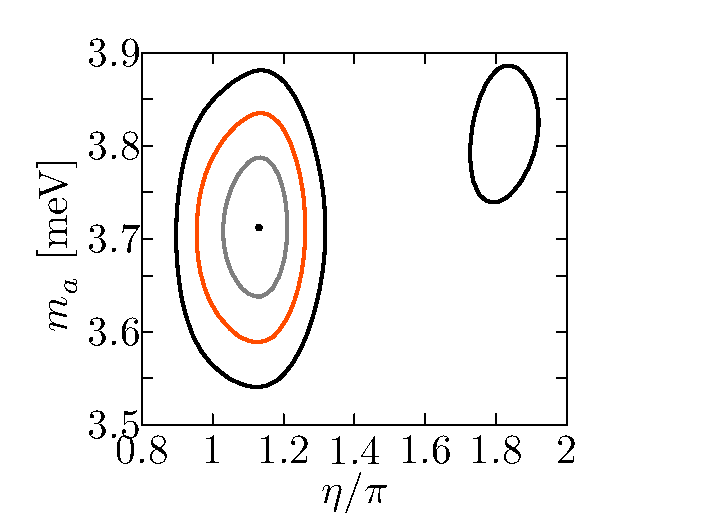
\includegraphics[width=0.32\textwidth]{figs/eta_ma.pdf}\hspace{-11mm}
 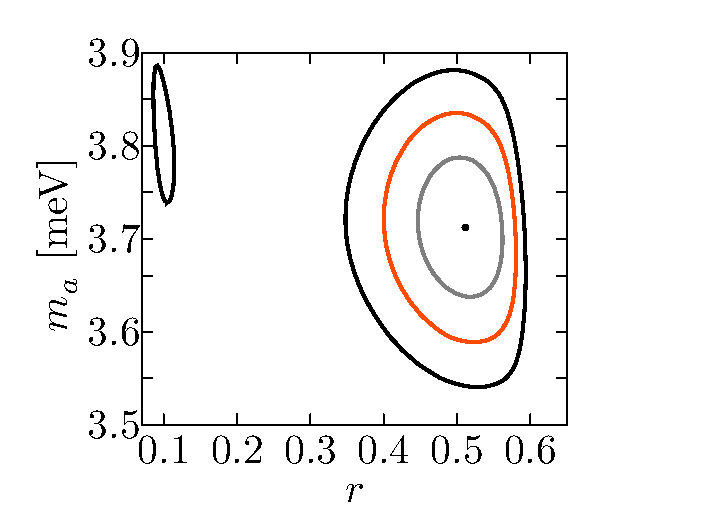
\includegraphics[width=0.32\textwidth]{figs/r_ma.pdf}
 \caption{\label{fig:model_2D}Precision measurements of any two model parameters at 3$\sigma$ confidence level in the framework of three neutrino oscillations taking uncertainties of the current global fit results, for MOMENT, at $1\sigma$ (gray), $2\sigma$ (orange), $3\sigma$ (black). True values for the model parameters are used $(x,~\eta,~r,~M_a)=(-3.65,~1.13\pi,~0.511,~3.71~\text{meV})$.}
\end{figure}


\subsection{Model testing}
\begin{figure}[!h]%
\centering
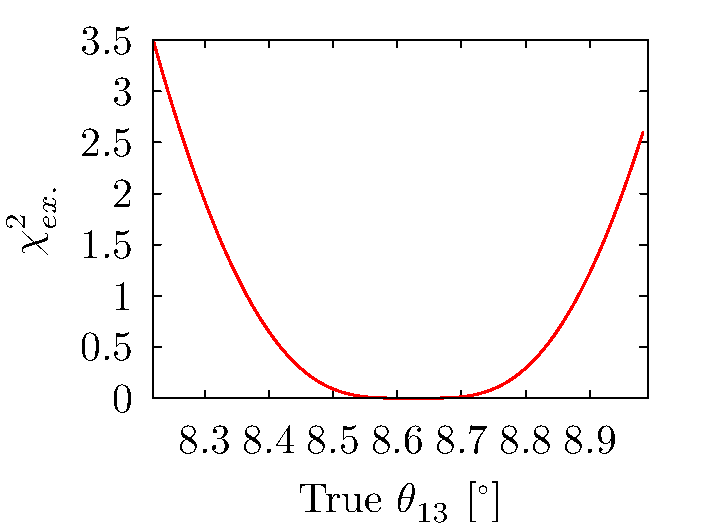
\includegraphics[width=2in]{figs/SR_th13.pdf}
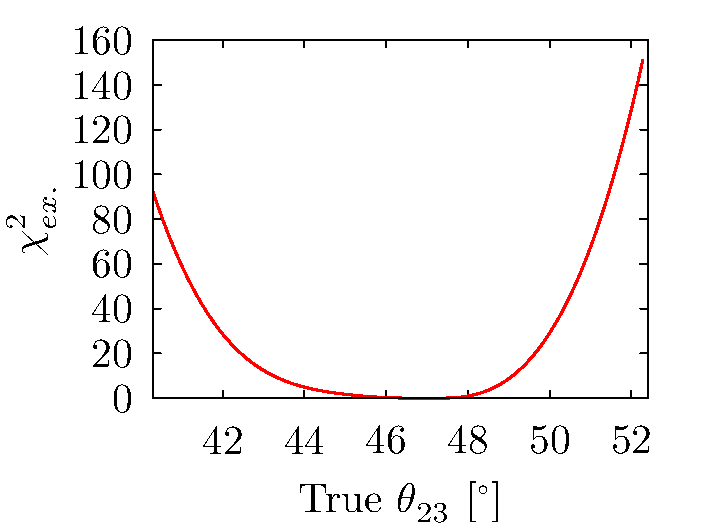
\includegraphics[width=2in]{figs/SR_th23.pdf}\\
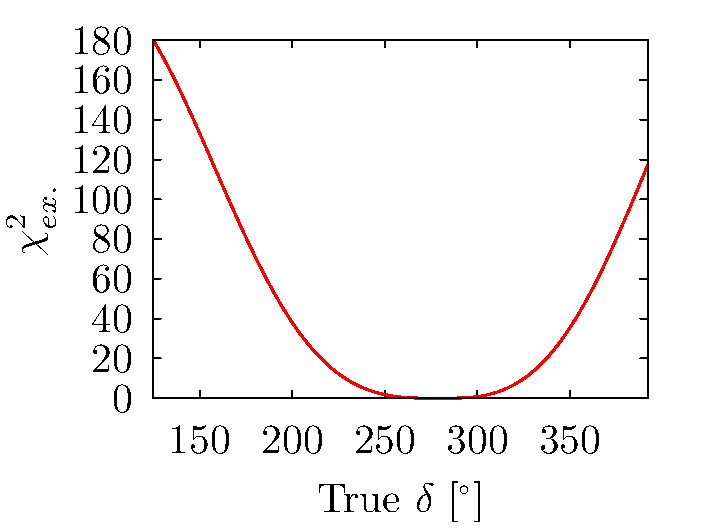
\includegraphics[width=2in]{figs/SR_dCP.pdf}
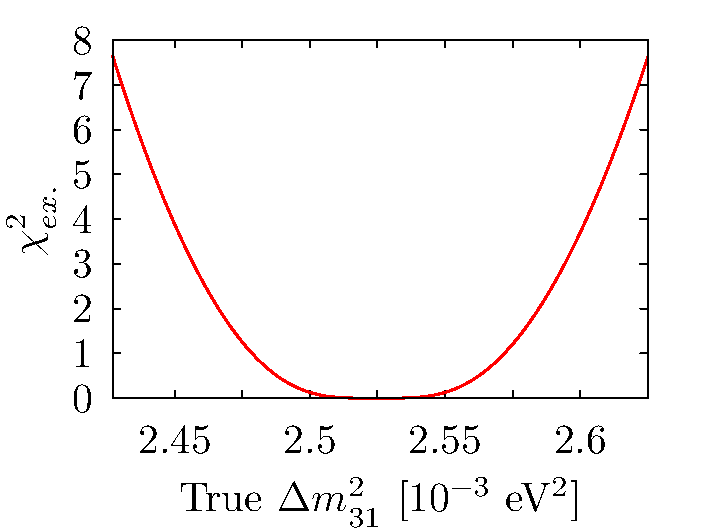
\includegraphics[width=2in]{figs/SR_ldm.pdf}
\caption{The $\chi^2_{ex.}$ value for tri-direct littlest seesaw model for $\theta_{13}$, $\theta_{23}$, $\delta$ and $\Delta m_{31}^2$. The range for each parameter is taken according to the $3\sigma$ uncertainty in NuFit4.0 results.}%
\label{fig:SR_1D}
\end{figure}

\begin{figure}[!h]
 \flushleft
%
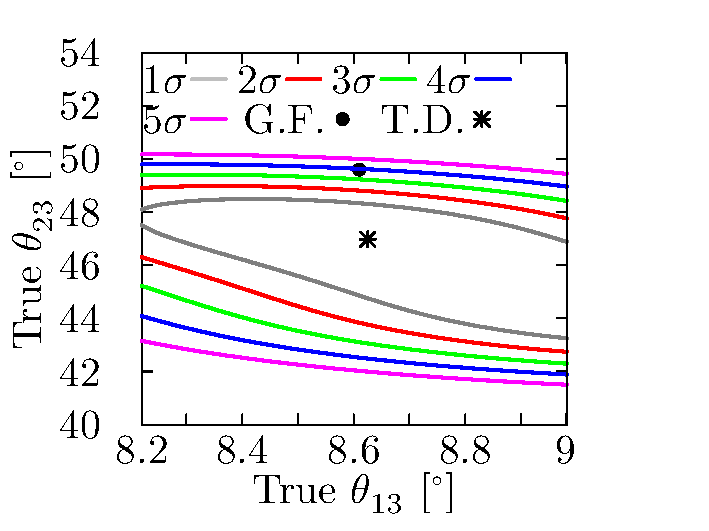
\includegraphics[width=0.32\textwidth]{figs/SR_th13_th23.pdf}$~~~~~~$\\
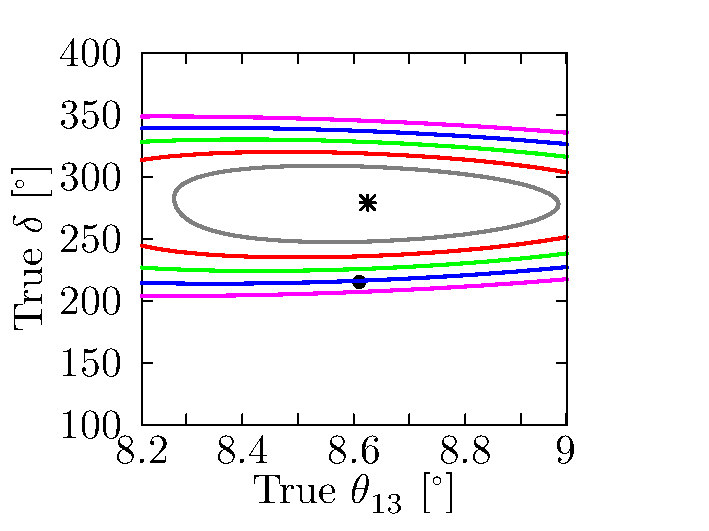
\includegraphics[width=0.32\textwidth]{figs/SR_th13_dCP.pdf}
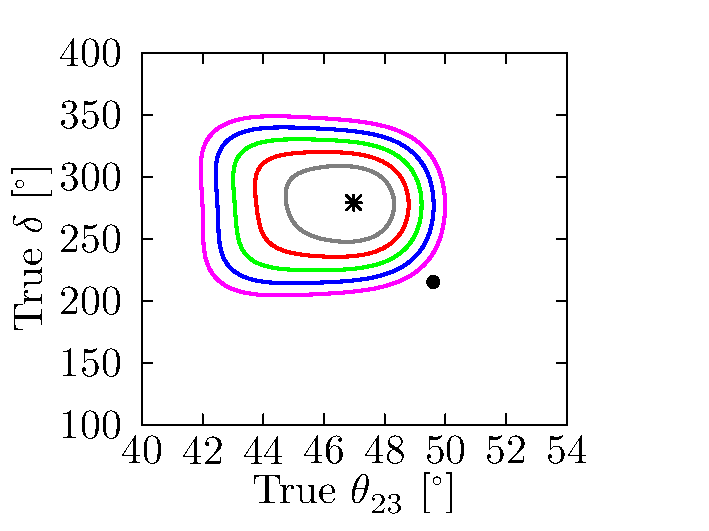
\includegraphics[width=0.32\textwidth]{figs/SR_th23_dCP.pdf}$~~~~~~$\\
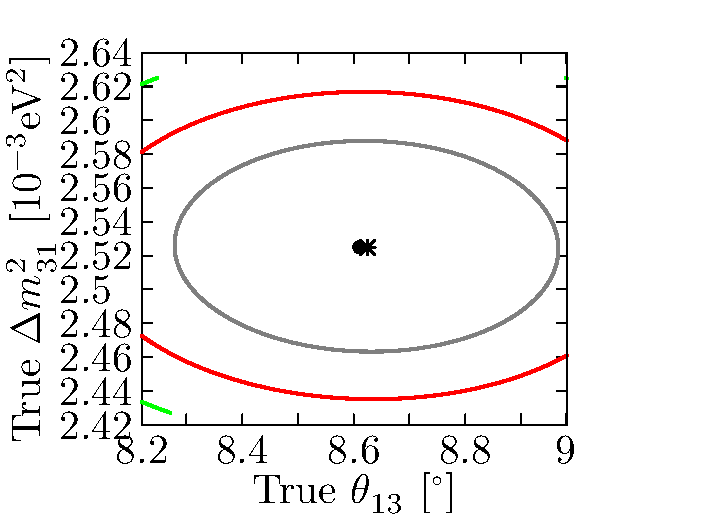
\includegraphics[width=0.32\textwidth]{figs/SR_th13_ldm.pdf}
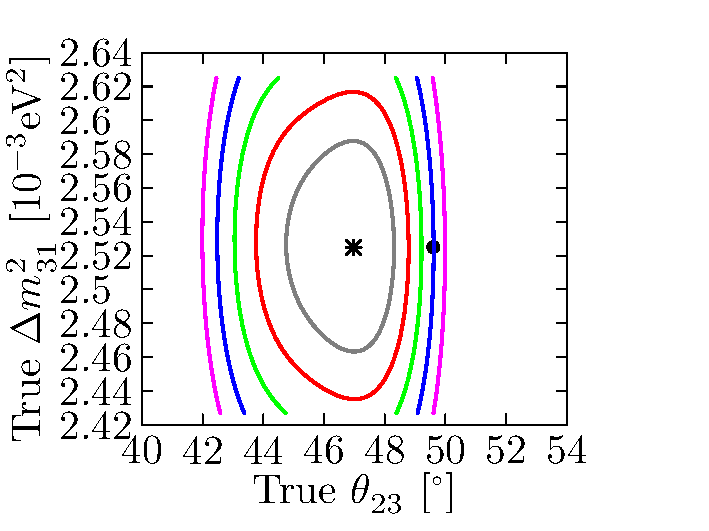
\includegraphics[width=0.32\textwidth]{figs/SR_th23_ldm.pdf}
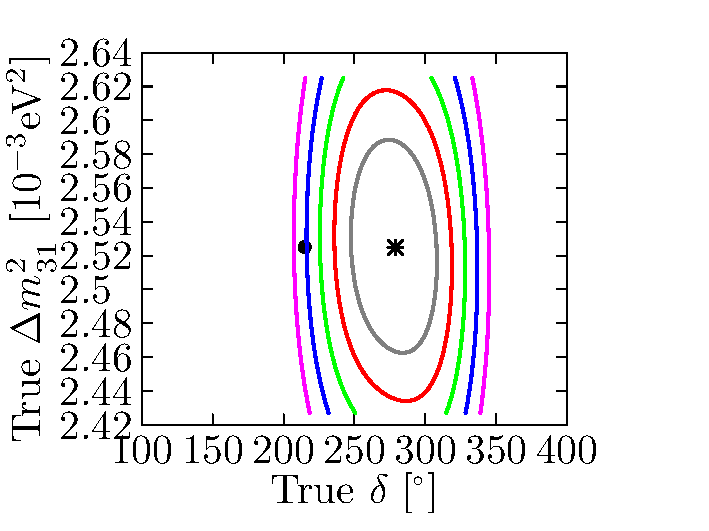
\includegraphics[width=0.32\textwidth]{figs/SR_dCP_ldm.pdf}
 \caption{\label{fig:SR_2D}The 2-D exclusion contour for tri-direct littlest seesaw model on the plane of any two true standard parameters, from $1\sigma$ to $5\sigma$. The range for each parameter is taken according to the $3\sigma$ uncertainty in NuFit4.0 results. The black dot denotes the best fit of NuFit4.0 results ($(\theta_{12},~\theta_{13},~\theta_{23},~\delta,~\Delta m_{21}^2,~\Delta m_{31}^2)=(33.82^\circ,~8.61^\circ,~49.6^\circ,~215^\circ,~7.39\times10^{-5}~\text{eV}^2,~2.525\times10^{-3}~\text{eV}^2)$), while the star is the prediction by the tri-direct littlest seesaw model with NuFit4.0 results ($(\theta_{12},~\theta_{13},~\theta_{23},~\delta,~\Delta m_{21}^2,~\Delta m_{31}^2)\sim(36.25^\circ,~8.63^\circ,~47^\circ,~279^\circ,~7.39\times10^{-5}~\text{eV}^2,~2.525\times10^{-3}~\text{eV}^2)$).}
\end{figure}



\section{Conclusion}

% BIBLIOGRAPHY
% use BIBTEX if you want
\bibliographystyle{JHEP}
\bibliography{FAS-GLoBES.bib}
\end{document}
